\chapter{Introduction}
\label{chap:introduction}

\section{Context}

Quality control plays an important role in large-scale software development. The number of coding errors are noticeably increasing with the number of contributors. The more developers work together on developing a software, the more versatile their coding styles and conventions are.

To ensure the quality of the source code, thus the software itself, and at the same time help developers with their tasks, the need arises for a solution continuously reviewing the code, searching for mistakes, and enforcing conventions.

\begin{figure}[!ht]
	\centering
	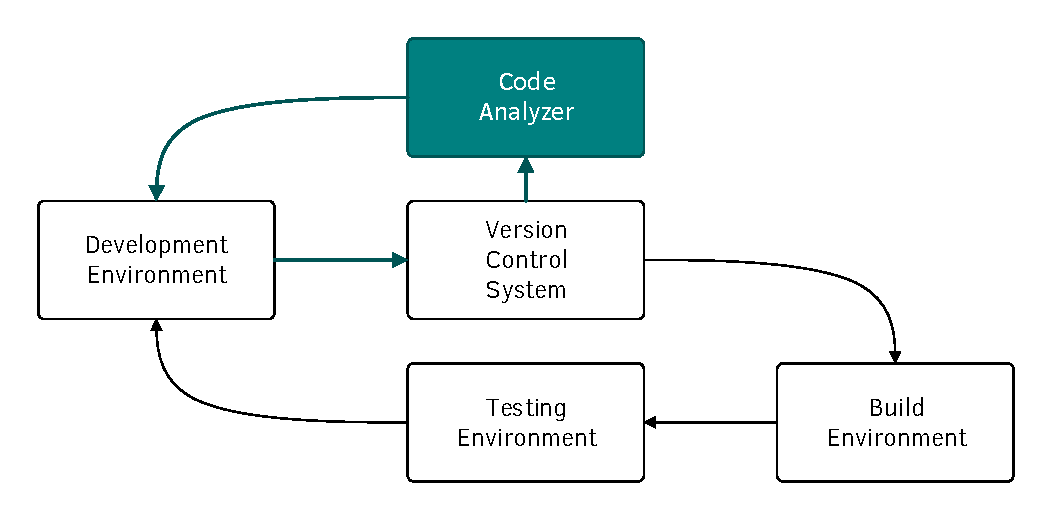
\includegraphics[height=6cm]{CI-workflow}
	\caption{Continuous Integration workflow extended with Static Analysis.}
	\label{fig:CI-workflow}
\end{figure}

Version control systems (VCS) and continuous integration (CI)~\cite{CI} are widely used tools of the modern software developers. \Cref{fig:CI-workflow} shows an extended version of the generally used continuous integration workflow.
The basic workflow consists of the following steps. The developer makes modifications to the codebase using their \textit{Development Environment}. The modifications are committed into a \textit{Version Control System}, and this commit triggers the \textit{Build Environment} to build the project. The \textit{Testing Environment} can then perform runtime tests on latest build of the project. After this process, the results --- build and test logs --- are presented to the developer.

These logs help the developers discover bugs and failures before the software is released for manual testing or production purposes. Producing this information and making sure the software is working as intended often and early in the development workflow is vital for agile development.

A proven method of enhancing software quality is utilizing static program analysis techniques supplementing the basic CI workflow. During this method, the code is analyzed without executing the application. In practice, this method is able to reveal problems that are undetectable with testing and thus is able to aid the developer in creating higher quality software.


\section{Problem Statement}

Static analysis methods verifying that the code is compliant with coding conventions are often time consuming and resource intensive in practice. The size of the codebase may require a scalable solution, especially for continuous integration purposes, since the entire verification process needs to be carried out on the whole codebase once it is (partially) modified.

A temporary solution to tackle this problem is to process the changes in batches. To save resources, static analysis runs are carried out for a joined group of changes, rather than for every individual commit.

In an ideal situation, even before committing the changes, the developers receive feedback about the problems their modifications would imply.


\section{Objectives and Contributions}

My main objective is to provide a solution for reducing the time required for global, codebase-level reevaluation of static analysis after a change occurs.

I aim to create a framework that transforms the whole source code repository into a graph representation and maintains it subsequently. It should perform code convention compliance checks, execute built-in static analysis tests and be extended with arbitrary tests by the user.

Incremental processing is one of the possible solutions for speeding up static analysis. Thus it should be able to process a subset of the repository, e.g. only the modifications introduced by the latest commit, then integrate the changes into the maintained representation. This way the system can process the modifications in a commit incrementally. After the initial query evaluation and report generation, consecutive runs can be executed significantly more efficiently.

The framework relies on two substantial technologies --- a source code parser and an adequate database solution --- and provides interfaces making integration possible with external tools, such as version control systems and integrated developer environments.


\section{Structure of the Thesis}

This thesis is structured as follows.
\Cref{chap:preliminaries} introduces the previously mentioned background technologies required and selected to build an incremental static analyzer.
\Cref{chap:background-and-related-work} details the various approaches and related researches.
\Cref{chap:overview-of-the-approach} shows the overview of my approach and gives detailed view of the main components of its architecture.
\Cref{chap:elaboration-of-the-workflow} presents the implementation of the framework, and discusses the steps of the analysis.
\Cref{chap:evaluation-of-the-prototype} demonstrates and evaluates the performance of the framework.
\Cref{chap:future-vision} reveals future vision ideas and possibilities.
\Cref{chap:conclusions} concludes the thesis.
